\documentclass[10pt]{article}
\usepackage{icmlko}

\icmlmeta{IP 파운데이션 월드모델}{44}{여섯 노트가 잡음을 조각하고 있었다}{신뢰구간을 붙이니 알고리즘 조정 셋은 전부 0을 포함하고 배선 하나만 살아남는다}

\begin{document}

\twocolumn[
\icmlheader

\begin{abstract}
노트 43은 판정 기준을 유의 개수에서 평균 순위 상관으로 옮기고 과거 결정 넷을
재감사했다. 그런데 근거로 쓴 차이가 0.3438 대 0.3516처럼 작았고 신뢰구간이
없었다. \textbf{자를 바꿨을 뿐 눈금을 읽지 않은 것이며, 그것은 노트 42가 지적한
것과 같은 실수다.} 연도 층화 짝지은 붓스트랩 300회로 구간을 붙였다. 결과가
가혹하다. \textbf{현행 평균 $\rho$ 자체의 95\% 구간이 [0.265, 0.406]으로 반폭이
0.071}인데, 노트 37부터 43까지 여섯 노트가 다툰 설정 간 차이는
0.009--0.022였다. 짝을 지어 분산을 상당히 걷어내도 알고리즘 조정 셋 ---
공통 축을 둘에서 셋으로($+$0.0215), 게임 매장축 끄기($+$0.0095), 이중 배선
($-$0.0094) --- 의 구간이 \textbf{전부 0을 포함한다}. 하나만 살아남았다.
노트 34가 도서 타깃 폭을 장르 수에서 판형으로 바꾼 것으로, 차이가
\textbf{$+$0.0939, 95\% 구간 [$+$0.046, $+$0.199]}다. 나머지의 네 배에서 열
배다. 노트 33이 관찰로 얻었던 문장 --- ``전이 알고리즘을 더 손볼 이유가 없다.
남은 일은 각 도메인에서 무엇을 어떻게 재느냐뿐이다'' --- 이 이제 구간으로
확증된다. 알고리즘 조정을 중단하고 배선과 데이터로 돌아간다.
\end{abstract}
]

\section{자를 바꾸고 눈금을 안 읽었다}

노트 42는 판정 도구가 눈금 조작에 속는 것을 잡아냈다. 노트 43은 도구를 바꿔
결정 넷을 재감사했다. 그런데 그 재감사가 쓴 근거는 이런 것이었다.

\begin{quote}\fontsize{9.5}{11.5}\selectfont
``게임 매장축을 끄면 0.3438에서 0.3516으로 오른다. 노트 37의 결정을 되돌린다.''
\end{quote}

0.008이다. 그것이 표본 요동보다 큰지 확인하지 않았다. \textbf{자를 바꿨을 뿐
눈금을 읽지 않은 것이고, 그것은 노트 42가 지적한 것과 같은 종류의 실수다.}

연도 층화 짝지은 붓스트랩 300회로 구간을 붙였다. 복제마다 도메인별 레코드를
복원추출하고, 축 유도와 인자 공간 추정을 다시 하고, 두 설정을 \emph{같은 복제
위에서} 계산해 차이를 기록한다. 짝을 짓는 이유는 노트 6에서 확립한 그대로다 ---
차이가 요동보다 훨씬 작을 때 독립 붓스트랩은 큰 분산 둘을 빼서 아무것도 못 본다.

\section{절대 구간이 얼마나 넓은가}

\begin{table}[t]
\centering\tsize
\caption{현행 설정의 평균 순위 상관.}
\begin{tabular}{lr}
\toprule
평균 $\rho$ & $+$0.3516 \\
95\% 붓스트랩 구간 & $[+0.265,\ +0.406]$ \\
구간 반폭 & \textbf{0.071} \\
\midrule
노트 37--43이 다툰 차이의 범위 & 0.009--0.022 \\
\bottomrule
\end{tabular}
\end{table}

반폭이 0.071인데 여섯 노트가 0.009에서 0.022 사이를 놓고 채택과 철회를 반복했다.
비율로 보면 논쟁의 대상이 불확실성의 8분의 1에서 3분의 1이었다.

짝을 지으면 공통 요동이 상쇄돼 차이의 구간은 훨씬 좁아진다. 그래도 충분하지
않았다.

\section{넷 중 하나만 살아남는다}

\begin{figure}[t]
\centering
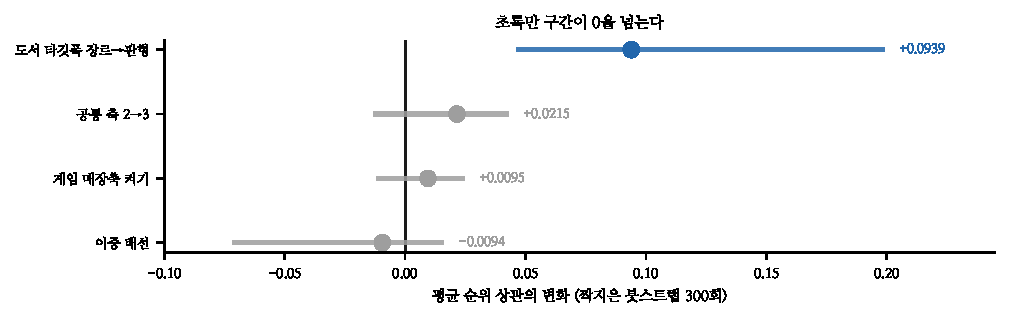
\includegraphics[width=\textwidth]{figs/forest.pdf}
\caption{짝지은 붓스트랩 300회. 가로선이 95\% 구간이다.}
\end{figure}

\begin{table}[t]
\centering\tsize
\caption{과거 결정의 효과와 구간.}
\begin{tabular}{lrrr}
\toprule
결정 & 차이 & 95\% 구간 & P($>$0) \\
\midrule
이중 배선(노트 39) & $-$0.0094 & $[-0.072, +0.016]$ & 0.11 \\
게임 매장축 끄기 & $+$0.0095 & $[-0.012, +0.025]$ & 0.80 \\
공통 축 2$\to$3(노트 37) & $+$0.0215 & $[-0.013, +0.043]$ & 0.86 \\
\midrule
\textbf{도서 타깃 폭 배선(노트 34)} & \textbf{$+$0.0939} &
$\mathbf{[+0.046, +0.199]}$ & \textbf{1.00} \\
\bottomrule
\end{tabular}
\end{table}

\begin{figure}[t]
\centering
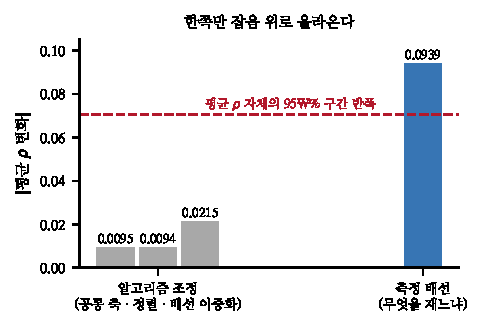
\includegraphics[width=\columnwidth]{figs/kinds.pdf}
\caption{결정 유형별 효과 크기. 점선이 평균 $\rho$ 자체의 구간 반폭이다.}
\end{figure}

\claimx{알고리즘 조정(공통 축 수, 정렬 방식, 역할별 배선, $\lambda$)의 효과는
현재 표본에서 전부 잡음과 구분되지 않는다. 측정 배선(무엇을 재느냐)만 구간이
0을 넘는다.}{도메인이나 표본이 늘어 구간이 좁아졌을 때 알고리즘 조정 중 어느
하나가 0을 넘으면 이 판정은 검정력 부족이었던 것이다 --- 효과가 없다는 증명이
아니라 못 봤다는 뜻이다.}

노트 34가 한 일은 이랬다. 도서 타깃 폭에 장르 수를 넣었는데 라벨과의 상관이
$-$0.073으로 무효였고, 개별 변수를 훑으니 판형이 가장 강해서($-$0.282) 바꿨다.
그 하나가 나머지 세 결정을 합친 것의 두 배 넘는 효과를 낸다.

\section{노트 33이 옳았다}

노트 33은 이렇게 끝났다.

\begin{quote}\fontsize{9.5}{11.5}\selectfont
``전이 알고리즘을 더 손볼 이유가 없다. 정렬 방법도, 출처 선택도, 공동 학습도
상한에 붙어 있는 값을 바꾸지 못한다. \textbf{남은 일은 각 도메인에서 무엇을
어떻게 재느냐뿐이다.}''
\end{quote}

그때는 관찰이었다 --- 전이 상관이 대상 자기 상관과 같다는 등식에서 추론한 것이다.
이제 구간으로 확증된다. 그리고 나는 그 문장을 쓴 뒤 여섯 노트 동안 정확히
금지된 일을 했다.

\begin{table}[t]
\centering\tsize
\caption{노트 33 이후의 작업 분류.}
\begin{tabular}{lll}
\toprule
노트 & 무엇을 했나 & 판정 \\
\midrule
34 & 도서 배선 & \textbf{살아남음} \\
35 & 도서 누출 제거 & 미검정 \\
36 & 고유 축 확대 & 기각(자체) \\
37 & 공통 축 확대 & 구간 0 포함 \\
38 & 상충 발견 & (관찰) \\
39 & 이중 배선 & 구간 0 포함 \\
40 & 다섯째 도메인 & 미검정 \\
41 & $\lambda$ 조정 & 철회(노트 42) \\
42 & 지표 결함 발견 & (도구) \\
43 & 지표 교체 & (도구) \\
\bottomrule
\end{tabular}
\end{table}

\paragraph{쓸모없지는 않았다}
노트 38·40의 상충, 노트 42의 지표 결함, 노트 43의 표본 크기 의존 --- 이것들은
채택 결정이 아니라 \emph{무엇이 작동하는지에 대한 지식}이고, 그 지식이 이 노트를
가능하게 했다. 다만 여섯 노트 중 성능을 실제로 올린 것은 하나도 없다.

\section{그래서 무엇을 하나}

\begin{quote}\fontsize{9.5}{11.5}\selectfont
알고리즘 조정을 중단한다. 남은 두 지렛대는 \textbf{배선}과 \textbf{데이터}다.
배선은 효과가 크고(구간 [$+$0.046, $+$0.199]) 검정도 싸다. 데이터는 구간
자체를 좁혀 앞으로의 모든 판정을 가능하게 한다.
\end{quote}

당장 할 수 있는 것이 셋이다.

\begin{enumerate}[leftmargin=1.3em,itemsep=0.15em]
\item 노트 35가 도서에서 한 것(전자책 누출 제거)을 나머지 네 도메인에서 반복한다.
      아직 구간을 붙이지 않았다.
\item 팝업 표본을 늘린다. 팝업이 대상일 때 귀무 SD가 0.334로 가장 넓다(n$=$75).
\item 남은 배선 후보를 순위 기준으로 전수 검정한다. 노트 38의 탐색은 인자 공간
      자기 상관을 목표로 했고 그것은 MAE 계열 지표였다.
\end{enumerate}

\section{한계}

\begin{itemize}[leftmargin=1.1em,itemsep=0.15em]
\item 붓스트랩 300회다. 구간 끝점이 $\pm$0.01쯤 흔들린다.
\item 복원추출을 레코드 단위로 했다. 같은 IP의 여러 레코드가 있으면 독립이
      아니므로 구간이 좁게 나온다(노트 7의 군집 문제).
\item 노트 35(도서 전자책 제외)와 노트 40(다섯째 도메인)은 구간을 붙이지 않았다.
      둘 다 표본 자체를 바꾸므로 짝지은 붓스트랩이 그대로 적용되지 않는다.
\item 네 결정을 각각 현행 대비로 쟀다. 조합 효과는 보지 않았다.
\item ``알고리즘 조정은 효과가 없다''가 아니라 ``현재 표본에서는 못 본다''가
      정확한 서술이다. 검정력 계산을 하지 않았다.
\end{itemize}

\section{다음}

\begin{enumerate}[leftmargin=1.3em,itemsep=0.15em]
\item 네 도메인에 결측 누출 검사를 순위 기준 구간과 함께 다시 돌린다.
\item 배선 후보 전수 검정 --- 순위 기준, 짝지은 붓스트랩.
\item 팝업 표본 확대 --- 구간을 좁히는 유일한 길.
\item 붓스트랩을 IP 군집 단위로 다시 짠다.
\end{enumerate}

\vspace{0.6em}
\hrule height 0.3pt
\vspace{0.5em}
{\footnotesize
\textbf{참고문헌}\\[0.3em]
Efron, B., Tibshirani, R. J. (1993). \emph{An Introduction to the Bootstrap}.
Chapman \& Hall.\\[0.15em]
Bouthillier, X. et al. (2021). Accounting for variance in machine learning
benchmarks. \emph{MLSys}, 3, 747--769.\\[0.15em]
Dror, R. et al. (2018). The hitchhiker's guide to testing statistical
significance in natural language processing. \emph{ACL}, 1383--1392.\\[0.15em]
Ben-David, S. et al. (2010). A theory of learning from different domains.
\emph{Machine Learning}, 79(1--2), 151--175.\\[0.15em]
Spearman, C. (1904). The proof and measurement of association between two things.
\emph{American Journal of Psychology}, 15(1), 72--101.
}

\end{document}
